\documentclass{article}

\usepackage[utf8]{inputenc}
\usepackage[T1]{fontenc}
\usepackage{hyperref}
\usepackage{tabularx}
\usepackage{array}
\usepackage{fancyhdr}
\usepackage{graphicx}
\usepackage[a4paper]{geometry}
\usepackage{multicol}
\usepackage{listings}
\usepackage{pgfplots}

\pgfplotsset{width=10cm,compat=1.9}

\title{Apprentissage automatique \\ Le jeu des bâtons}
\author{par Camille Leplumey et Geoffrey Spaur}
\date{31 mars 2017}
\pagestyle{fancy}
\lhead{Apprentissage automatique - Le jeu des bâtons \\ \textbf{M1GIL} - Camille Leplumey et Geoffrey Spaur}
\rhead{
\includegraphics[scale=0.5]{logo_univ_rouen.png}}
\setlength{\headsep}{1cm}
\begin{document}

\maketitle
\newpage
\tableofcontents{}
\newpage
\section{Mode \emph{easy}}
  Le CPU joue aléatoirement sans prendre de décisions. Il est donc possible qu'il perde bêtement.
\section{Mode \emph{medium}}
  Le mode medium ne constitue en rien à de l'apprentissage. En effet nous codons les derniers coups que doit
  jouer le CPU. Le résultat sera donc identique à chaque parties sur les derniers coups et aléatoire sur les autres coups.
\section{Mode \emph{hard}}
  \paragraph{}
    Ici en entraînant le CPU contre lui même en mode \emph{hard}, il va apprendre la stratégie gagnante par lui même sans aide extérieur. 
    C'est un apprentissage non supervisé. Nous utilisons cette méthode car nous pouvons l'automatiser facilement.
  \paragraph{}
    \begin{tikzpicture}
     \begin{axis}[
	title={Évolution du taux moyen de réussite contre un joueur hard sans changement de rôle},
	ylabel={Taux de réussite en pourcentage },
	xlabel={Nombre de parties},
	ymin=0, ymax=100,ytick={0,20,40,60,80,100},
	xmin=0, xmax=7,xtick={0,1,2,3,4,5,6,7},
	xticklabels={0,100,500,1.000,5.000,10.000,50.000,100.000},
	scaled ticks=false,
	tick label style={/pgf/number format/fixed}, smooth,
	legend entries={Premier joueur,Second joueur},
	legend style={at={(0,1)},anchor=north west},
	legend cell align={left}
    ]
    
    \addplot[color=blue,mark=square,]
	coordinates {(0,50)(1,47)(2, 60)(3, 68)(4, 81)(5, 89)(6, 95)(7, 97)};
    \addplot[color=gray,mark=square,]
	coordinates {(0,50)(1,45)(2, 39)(3, 33)(4, 16)(5, 12)(6, 4)(7, 3)};
  
    \end{axis}
    \end{tikzpicture}\\
    Nous voyons ici qu'en jouant 800 parties, le CPU obtiendrais une moyenne de 65\% de réussite. Nous de
    plus affirmer qu'à partir de 50.000 parties jouées, le CPU ne fera quasiment plus d'erreurs.
  \paragraph{}
    \begin{tikzpicture}
     \begin{axis}[
	title={Évolution du taux moyen de réussite contre un joueur \textbf{easy} sans changement de rôle},
	ylabel={Taux de réussite en pourcentage },
	xlabel={Nombre de parties},
	ymin=0, ymax=100,ytick={0,20,40,60,80,100},
	xmin=0, xmax=7,xtick={0,1,2,3,4,5,6,7},
	xticklabels={0,100,500,1.000,5.000,10.000,50.000,100.000},
	scaled ticks=false,
	tick label style={/pgf/number format/fixed},
	legend entries={Second joueur easy,Second joueur medium,Second joueur hard},
	legend style={at={(0,1)},anchor=north west},
	legend cell align={left}
    ]
    \addplot[color=green,mark=square,]
	coordinates {(0,50)(1,50)(2, 50)(3, 50)(4, 50)(5, 50)(6, 50)(7, 50)};
    \addplot[color=blue,mark=square,]
	coordinates {(0,6)(1,6)(2, 6)(3, 6)(4, 6)(5, 6)(6, 6)(7, 6)};
    \addplot[color=red,mark=square,]
	coordinates {(0,50)(1,3)(2, 2)(3, 1)(4, 1)(5, 1)(6, 0.5)(7, 0.5)};
  
    \end{axis}
    \end{tikzpicture}
    
  \paragraph{}
    \begin{tikzpicture}
     \begin{axis}[
	title={Évolution du taux moyen de réussite contre un joueur \textbf{medium} sans changement de rôle},
	ylabel={Taux de réussite en pourcentage },
	xlabel={Nombre de parties},
	ymin=0, ymax=100,ytick={0,20,40,60,80,100},
	xmin=0, xmax=7,xtick={0,1,2,3,4,5,6,7},
	xticklabels={0,100,500,1.000,5.000,10.000,50.000,100.000},
	scaled ticks=false,
	tick label style={/pgf/number format/fixed}, smooth,
	legend entries={Second joueur easy,Second joueur medium,Second joueur hard},
	legend style={at={(0,0)},anchor=south west},
	legend cell align={left}
    ]
    \addplot[color=green,mark=square,]
	coordinates {(0,95)(1,95)(2, 94)(3, 94)(4, 94)(5, 95)(6, 95)(7, 95)};
    \addplot[color=blue,mark=square,]
	coordinates {(0,50)(1,51)(2, 50)(3, 50)(4, 51)(5, 50)(6, 50)(7, 50)};
    \addplot[color=red,mark=square,]
	coordinates {(0,95)(1,50)(2, 27)(3, 21)(4, 11)(5, 11)(6, 7)(7, 5)};
  
    \end{axis}
    \end{tikzpicture}
  
  \paragraph{}
    \begin{tikzpicture}
     \begin{axis}[
	title={Évolution du taux moyen de réussite contre un joueur \textbf{hard} sans changement de rôle},
	ylabel={Taux de réussite en pourcentage },
	xlabel={Nombre de parties},
	ymin=0, ymax=100,ytick={0,20,40,60,80,100},
	xmin=0, xmax=7,xtick={0,1,2,3,4,5,6,7},
	xticklabels={0,100,500,1.000,5.000,10.000,50.000,100.000},
	scaled ticks=false,
	tick label style={/pgf/number format/fixed}, smooth,
	legend entries={Second joueur easy,Second joueur medium,Second joueur hard},
	legend style={at={(1,0)},anchor=south east},
	legend cell align={left}
    ]
    \addplot[color=green,mark=square,]
	coordinates {(0,50)(1,90)(2, 96)(3, 97)(4, 98)(5, 98)(6, 99)(7, 99.5)};
    \addplot[color=blue,mark=square,]
	coordinates {(0,5)(1,50)(2, 76)(3, 81)(4, 89)(5, 90)(6, 93)(7, 94)};
    \addplot[color=red,mark=square,]
	coordinates {(0,50)(1,47)(2, 60)(3, 68)(4, 81)(5, 89)(6, 95)(7, 97)};
  
    \end{axis}
    \end{tikzpicture}

  \paragraph{}
    Pour conclure, si nous voulons jouer contre le CPU en mode \emph{hard}, il sera toujours possible de gagner.
    En effet le CPU choisi aléatoirement parmi ces connexions en favorisant les connexions à fort poids. 
    Néanmoins la chance que le CPU choisisse une connexion perdante sera toujours non nul. Même si le CPU est bien entraîné,
    avec de la patience, il sera toujours possible de gagner une partie contre lui.
  
\end{document}